\documentclass[10pt]{article}
\usepackage{polski}
\usepackage[utf8]{inputenc}
\usepackage{amsmath}
\usepackage{amsfonts}
\usepackage{tabto,lipsum}
\usepackage{calc}
\usepackage{xcolor}
\usepackage{graphicx}
\graphicspath{ {./img/} }
\usepackage{shadowtext}
\usepackage{hyperref}
\hypersetup{%
  colorlinks=false,% hyperlinks will be black
  linkbordercolor=red,% hyperlink borders will be red
  pdfborderstyle={/S/U/W 1}% border style will be underline of width 1pt
}
\usepackage[margin=1.5cm]{geometry}
\usepackage{algpseudocode}
\usepackage{algorithm}
\usepackage{listings}
\usepackage{ulem}
\usepackage{cancel}
\usepackage{adjustbox}
\usepackage{pgfplots}
\usepackage{bm}

\PassOptionsToPackage{usenames,dvipsnames,svgnames}{xcolor}
\usepackage{tikz}
\usetikzlibrary{arrows,positioning,automata}

\linespread{1.3}

\title{Obliczenia Naukowe,\\Laboratorium, Lista 3}
\author{Jerzy Wroczyński}
\date{2020-11-22}

\begin{document}

\maketitle

\section{Zadanie 1.}

\subsection{Opis problemu}

Napisać funkcję rozwiązującą równanie $f(x) = 0$ metodą bisekcji.

\subsubsection{Dane wejściowe}

\begin{itemize}
    \item \texttt{f} — funkcja $f$ w postaci anonimowej funkcji
    \item \texttt{a,b} — liczby typu \texttt{Float64} określające końce przedziału początkowego
    \item \texttt{delta, epsilon} — liczby typu \texttt{Float64} określające dokładności obliczeń
\end{itemize}

\subsubsection{Dane wyjściowe}

Czwórka wartości \texttt{(r,v,it,err)}.

\begin{itemize}
    \item \texttt{r} — przybliżenie pierwiastka równania $f(x) = 0$
    \item \texttt{v} — wartość funkcji w $r$
    \item \texttt{it} — liczba wykonanych iteracji
    \item \texttt{err} — sygnalizacja błędu, możliwe wartości:
    \begin{itemize}
        \item \texttt{0} — brak błędu
        \item \texttt{1} — funkcja nie zmienia znaku w przedziale $[a;b]$
    \end{itemize}
\end{itemize}

\subsection{Rozwiązanie}

Kod źródłowy znajduje się w pliku \texttt{code/iterative-methods.jl} jako funkcja \texttt{mbisekcji}.

\subsection{Opis metody}

Mając pewien przedział $[a;b]$ gdzie $f(a) \cdot f(b) = -1$ (mamy inne znaki wartości funkcji w granicach przedziału) mamy pewność, że funkcja ma w tym przedziale miejsce zerowe. Idea jest taka: dzielimy przedział na dwie części (wyznaczając środek przedziału) i sprawdzamy gdzie mamy spełniony warunek $f(a') \cdot f(b') = -1$ w nowym przedziale $[a';b']$ będący połówką poprzedniego przedziału $[a;b]$.

\noindent Powtarzamy czynność aż nie osiągniemy oczekiwanej precyzji (określonej przez odpowiednie argumenty ze specyfikacji), czyli $|b-a| < \delta$ lub $|f(c)| < \epsilon$ gdzie $c$ to środek przedziału.

Oczywiście, żeby metoda działała poprawnie zadana funkcja wejściowa musi być ciągła w tym przedziale.

\begin{figure}[H]
    \centering
    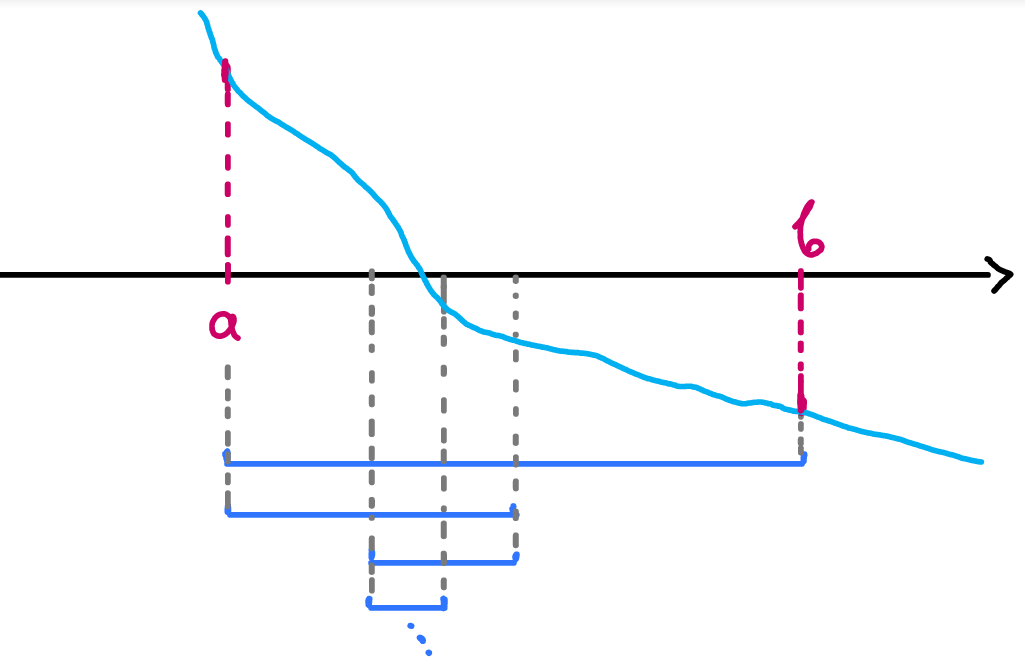
\includegraphics{metoda-bisekcji.png}
    \caption{Przykład zastosowania metody bisekcji, kilka iteracji zawężania przedziału}
\end{figure}

\subsection{Opis algorytmu}

Algorytm bisekcji opisuje poniższa lista kroków (przyjmujemy wcześniej opisaną specyfikację danych wejściowych i wyjściowych):

\begin{algorithm}[H]
    \begin{algorithmic}[1]
      \State $u \gets f(a)$\label{1.alg.begin}
      \State $v \gets f(b)$
      \State $e \gets (b-a)$\label{1.alg.begin.end}
      \If{$\operatorname{sgn}(u) = \operatorname{sgn}(v)$}\label{1.alg.first-if}
        \State \Return $(a, u, 0, 1)$
      \EndIf
      \For{$k \gets 0\dots$\texttt{MAX\_ITERATIONS}}\label{1.alg.for.begin}
        \State $e \gets \frac{e}{2}$\label{1.alg.for.division}
        \State $c \gets a + e$
        \State $w \gets f(c)$\label{1.alg.for.division-end}
        \If{$|e| < \delta$ or $|w| < \epsilon$}\label{1.alg.for.outif}
            \State \Return $(c, w, k, 0)$
        \EndIf

        \If{$\operatorname{sgn}(w) \neq \operatorname{sgn}(u)$}\label{1.alg.for.choose}
            \State $b \gets c$
            \State $v \gets w$
        \Else
            \State $a \gets c$
            \State $u \gets w$
        \EndIf\label{1.alg.for.choose.end}
      \EndFor
    \end{algorithmic}
\end{algorithm}

W linijkach \ref{1.alg.begin}–\ref{1.alg.begin.end} przygotowujemy program do działania (obliczamy wartości w punktach granicznych przedziału początkowego). W linijce \ref{1.alg.first-if} mamy pierwsze sprawdzenie poprawności danych. Jeśli w podanym przedziale $[a;b]$ podana funkcja nie zmienia znaku — odrzucamy, zwracamy wynik z zaznaczeniem błędu.

W linijce \ref{1.alg.for.begin} zaczynamy iterować. Najpierw dzielimy przedział na dwie części (\ref{1.alg.for.division}), ale jeszcze przed wyborem, którą część bierzemy, sprawdzamy jeszcze czy nie spełniliśmy warunku wyjściowego (\ref{1.alg.for.outif}).

Na koniec wybieramy oczywiście tę połowę przedziału (w celu zdefiniowania nowego przedziału do kolejnych iteracji), która zawiera miejsce zerowe (mamy różne znaki wartości funkcji $f$ w granicach nowego przedziału).

\section{Zadanie 2.}\label{2.}

\subsection{Opis problemu}

Napisać funkcję rozwiązującą równanie $f(x) = 0$ metodą Newtona.

\subsubsection{Dane wejściowe}

\begin{itemize}
    \item \texttt{f} — funkcja $f$ w postaci anonimowej funkcji
    \item \texttt{pf} — pochodna funkcji $f$ w postaci anonimowej funkcji
    \item \texttt{x0} — przybliżenie początkowe
    \item \texttt{delta, epsilon} — liczby typu \texttt{Float64} określające dokładności obliczeń
    \item \texttt{maxit} — liczba całkowita określająca dopuszczalną liczbę iteracji
\end{itemize}

\subsubsection{Dane wyjściowe}

Czwórka wartości \texttt{(r,v,it,err)}.

\begin{itemize}
    \item \texttt{r} — przybliżenie pierwiastka równania $f(x) = 0$
    \item \texttt{v} — wartość funkcji w $r$
    \item \texttt{it} — liczba wykonanych iteracji
    \item \texttt{err} — sygnalizacja błędu, możliwe wartości:
    \begin{itemize}
        \item \texttt{0} — metoda zbieżna
        \item \texttt{1} — nie osiągnięto wymaganej dokładności w \texttt{maxit} iteracji
        \item \texttt{2} — pochodna bliska zeru
    \end{itemize}
\end{itemize}

\subsection{Rozwiązanie}

Kod źródłowy znajduje się w pliku \texttt{code/iterative-methods.jl} jako funkcja \texttt{mstycznych}.

\subsection{Opis metody}

Idea metody Newtona (metody stycznych) opiera się na linearyzacji funkcji czyli zastąpieniu funkcji wejściowej $f$ funkcją liniową. Chcemy uzyskać funkcję liniową, która w jakiś sposób przybliża prawdziwą funkcję. Wykorzystujemy tutaj rozwinięcie w szereg Taylora, przy czym bierzemy tylko dwa pierwsze wyrazy. Ta metoda jest nazywana metodą stycznej, bo właśnie tym jest ta nowa funkcja (i właśnie dlatego też potrzebujemy pochodnej funkcji wejściowej, bo pochodna właśnie określa styczną do funkcji początkowej w danym punkcie).

Możemy sobie pozwolić na wzięcie tylko dwóch pierwszych wyrazów szeregu Taylora pod warunkiem, że to odchylenie między punktem początkowym a docelowym nie jest duże.

Metoda Newtona zaczyna od jakiegoś początkowego punktu $x_n$, który jest w pewnej odległości od szukanego punktu. Czyli mamy od tego $x_n$ pewne odchylenie. Wówczas mamy
$$
f(\tilde{r}) \approx f(x_n) + f'(x_n) \cdot (\tilde{r} - x_n)
$$
korzystając z dwóch pierwszych wyrazów szeregu Taylora. Oczywiście $f(\tilde{r})$ jest równe zero (szukamy miejsc zerowych), wówczas
$$
0 \approx f(x_n) + f'(x_n) \cdot (\tilde{r} - x_n)
$$
co po pewnych przekształceniach daje nam
$$
\tilde{r} \approx x_n - \frac{f(x_n)}{f'(x_n)}.
$$

Oczywiście, mając obliczony przybliżony kolejny punkt możemy zrobić znowu to samo, żeby się zbliżyć do rozwiązania. Dlatego definiujemy wzór rekurencyjny
\begin{equation}
    x_{n+1} = x_n - \frac{f(x_n)}{f'(x_n)},
    \label{2.recursion}
\end{equation}
który tworzy nasz ciąg coraz to lepszych wyników. Oczywiście musimy też zadbać o to, żeby „wystartować” w miejscu niedalekim od szukanego zera funkcji, żeby metoda ta miała szansę znaleźć to miejsce zerowe.

Tak samo jak w przypadku metody bisekcji — zatrzymujemy się wtedy kiedy osiągnęliśmy zadaną precyzję: $|x_{n+1} - x_n| < \delta \lor |f(x_{n+1})| < \epsilon$.

Minusem tej metody, że potrzebujemy mieć zdefiniowaną pochodną zadanej funkcji wejściowej.

\begin{figure}[H]
    \centering
    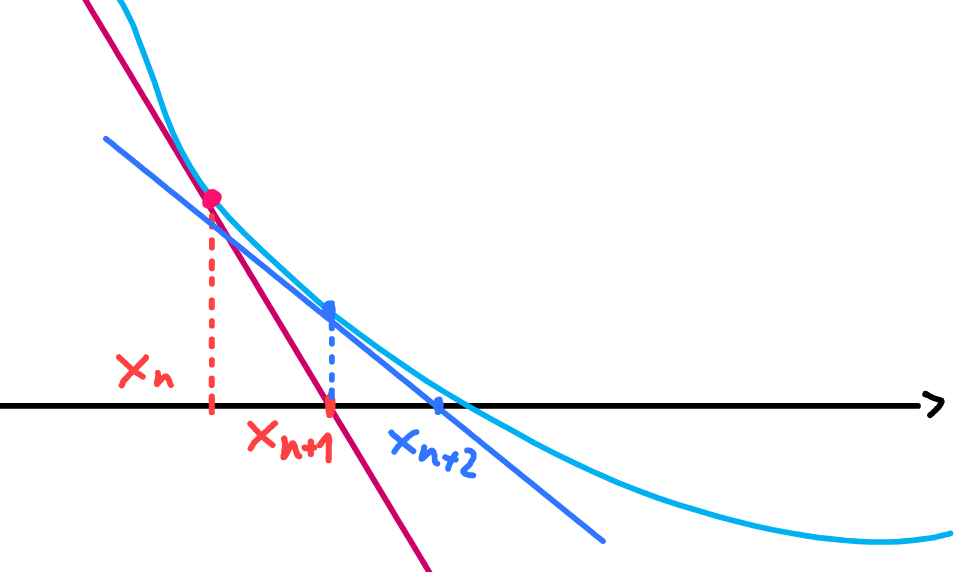
\includegraphics{metoda-newtona.png}
    \caption{Przykład zastosowania metody Newtona}
\end{figure}

\subsection{Opis Algorytmu}

Algorytm wykorzystujący metodę Newtona opisuje poniższa lista kroków (przyjmujemy wcześniej opisaną specyfikację danych wejściowych i wyjściowych):

\begin{algorithm}[H]
    \begin{algorithmic}[1]
      \State $v \gets f(x_0)$\label{2.alg.begin}
      \If{$|v| < \epsilon$}\label{2.alg.firstif}
        \State \Return $(x_0, v, 0, 0)$
      \EndIf
      \State $x_{n} \gets x_0$
      \For{$k \gets 0\dots$\texttt{maxit}}\label{2.alg.for.begin}
        \State $x_{n+1} \gets x_n - \frac{v}{f'(x_n)}$\label{2.alg.for.rec-step}
        \State $v \gets f(x_{n+1})$

        \If{$f'(x_n) <$ \texttt{NEAR\_ZERO}}\label{2.alg.for.derivative-near-zero}
            \State \Return $(x_n, f(x_n), k, 2)$
        \EndIf

        \If{$|x_{n+1} - x_n| < \delta \lor |v| < \epsilon$}\label{2.alg.for.outif}
            \State \Return $(x_{n+1}, v, k, 0)$
        \EndIf
        \State $x_n \gets x_{n+1}$\label{2.alg.for.continue}
      \EndFor

      \State \Return $(x_{n+1}, v, k, 1)$
    \end{algorithmic}
\end{algorithm}

Algorytm najpierw sprawdza czy wynik początkowy nie jest już wystarczający, biorąc pod uwagę podaną precyzję (\ref{2.alg.firstif}). Następnie przechodzimy do iterowania kolejnych wyrazów naszego ciągu, który zbiega do faktycznego rozwiązania. W środku pętli \ref{2.alg.for.begin} oprócz sprawdzania czy nie dotarliśmy do wyniku o żądanej precyzji \ref{2.alg.for.outif}, ale też patrzymy czy wartość pochodnej nie jest bliska zeru — jeżeli jest to przerywamy program i zwracamy informację z błędem o określonym kodzie ze specyfikacji.

W linijce \ref{2.alg.for.outif} sprawdzamy, czy żądana precyzja została osiągnięta — jeśli tak to zwracamy aktualnie wyliczoną wartość. W przeciwnym przypadku w linijce \ref{2.alg.for.continue} „przesuwamy” wartość wyrazu ciągu i kontynuujemy iterowanie.

Jeśli przekroczymy liczbę iteracji, zwracamy ostanią wyliczoną wartość wraz z błędem \texttt{1} zgodnie ze specyfikacją.


\section{Zadanie 3.}

\subsection{Opis problemu}

Napisać funkcję rozwiązującą równanie $f(x) = 0$ metodą siecznych.

\subsubsection{Dane wejściowe}

\begin{itemize}
    \item \texttt{f} — funkcja $f$ w postaci anonimowej funkcji
    \item \texttt{x0,x1} — przybliżenia początkowe
    \item \texttt{delta, epsilon} — liczby typu \texttt{Float64} określające dokładności obliczeń
    \item \texttt{maxit} — liczba całkowita określająca dopuszczalną liczbę iteracji
\end{itemize}

\subsubsection{Dane wyjściowe}

Czwórka wartości \texttt{(r,v,it,err)}.

\begin{itemize}
    \item \texttt{r} — przybliżenie pierwiastka równania $f(x) = 0$
    \item \texttt{v} — wartość funkcji w $r$
    \item \texttt{it} — liczba wykonanych iteracji
    \item \texttt{err} — sygnalizacja błędu, możliwe wartości:
    \begin{itemize}
        \item \texttt{0} — metoda zbieżna
        \item \texttt{1} — nie osiągnięto wymaganej dokładności w \texttt{maxit} iteracji
    \end{itemize}
\end{itemize}

\subsection{Rozwiązanie}

Kod źródłowy znajduje się w pliku \texttt{code/iterative-methods.jl} jako funkcja \texttt{msiecznych}.

\subsection{Opis metody}

Metoda siecznych jest nieco zmienioną wersją metody Newtona. Po pierwsze mamy zmianę w danych wejściowych do algorytmu, a po drugie mamy inną interpretację geometryczną tego podejścia.

Zamiast podawania dodatkowo pochodnej funkcji, której chcemy znaleźć pierwiastek, podajemy dwa przybliżone punkty i tak naprawdę to sami obliczamy taką pseudo-pochodną ze wzoru z definicji na pochodną:
$$
f'(x) = \frac{f(x) - f(x + h)}{h}.
$$
Oczywiście, oryginalnie mówimy o pochodnej kiedy $h$ dąży do zera. Tutaj, punkty $x$, $(x+h)$ są jednak od siebie relatywnie daleko — dlatego też nie mówimy już o stycznej, a raczej właśnie o siecznej.

\begin{figure}[H]
    \centering
    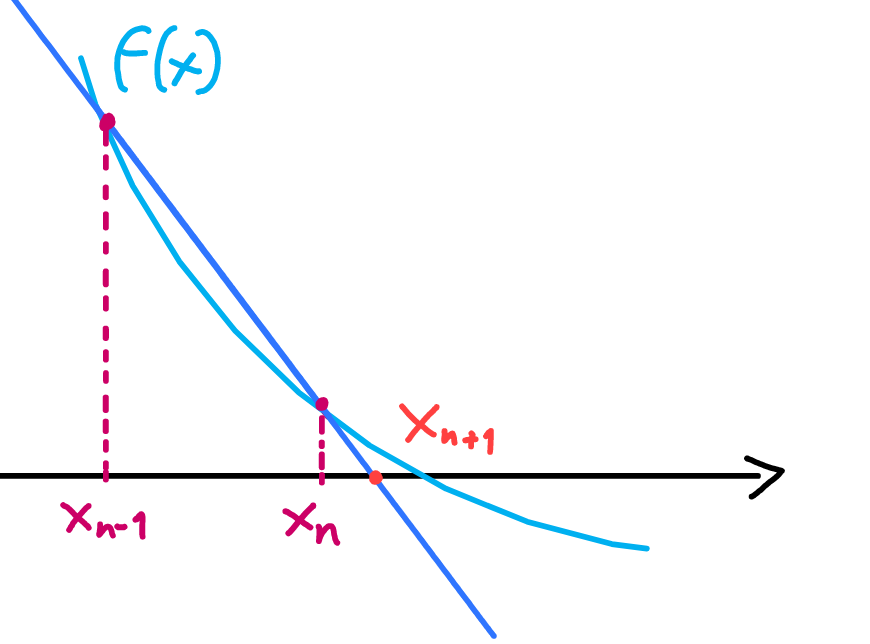
\includegraphics{metoda-siecznych.png}
    \caption{Przykład zastosowania metody siecznych}
\end{figure}

Zdefiniujmy naszą pochodną w tych nowych warunkach:
$$
f'(x_n) \approx \frac{f(x_n) - f(x_{n-1})}{x_n - x_{n-1}}
$$
i skorzystajmy ze wzoru \ref{2.recursion}, który w zadaniu \ref{2.}. definiował nam kolejne wyrazy — jednakże tym razem wzór na kolejny wyraz ciągu jest uzależniony od dwóch poprzednich:
\begin{equation}
    x_{n+1} = x_n - \frac{f(x_n)}{f'(x_n)} = x_n - f(x_n) \cdot \frac{x_n - x_{n-1}}{f(x_n) - f(x_{n-1})}
\end{equation}

Tak samo jak w poprzednich metodach — zatrzymujemy się wtedy kiedy osiągnęliśmy zadaną precyzję: $|x_{n+1} - x_n| < \delta \lor |f(x_{n+1})| < \epsilon$.

\subsection{Opis algorytmu}\label{3.alg}

Algorytm wykorzystujący metodę siecznych opisuje poniższa lista kroków (przyjmujemy wcześniej opisaną specyfikację danych wejściowych i wyjściowych):

\begin{algorithm}[H]
    \begin{algorithmic}[1]
      \State $v \gets f(x_0)$\label{3.alg.begin}
      \State $w \gets f(x_1)$
      \State $a \gets x_0$
      \State $b \gets x_1$\label{3.alg.begin.end}
      \For{$k \gets 0\dots$\texttt{maxit}}\label{3.alg.for.begin}
        \If{$|v| > |w|$}\label{3.alg.for.firstif}
            \State $a,b \gets b,a$
            \State $v,w \gets w,v$
        \EndIf
        \State $d \gets \frac{b - a}{w - v}$\label{3.alg.for.recursive.begin}
        \State $b \gets a$
        \State $w \gets v$
        \State $a \gets a - d \cdot v$
        \State $v \gets f(a)$\label{3.alg.for.recursive.end}
        \If{$|v| < \epsilon \lor |b-a| < \delta$}\label{3.alg.for.outif}
            \State \Return $(a, v, k, 0)$
        \EndIf
      \EndFor

      \State \Return $(a, v, k, 1)$\label{3.alg.errorif}
    \end{algorithmic}
\end{algorithm}

W linijkach \ref{3.alg.begin}–\ref{3.alg.begin.end} przygotowujemy dane do działania algorytmu — obliczamy wartości w danych punktach początkowych oraz wkładamy pierwsze dwie aproksymacje do odpowiednich zmiennych.

W linijce \ref{3.alg.for.begin} zaczynamy iterować. W środku pętli upewniamy się, że mamy zachowany porządek obliczonych wartości (\ref{3.alg.for.firstif}). Dzięki temu wartości kolejnych wyrazów ciągu nie będą rosnąć — a tego chcemy, bo szukamy miejsca zerowego.

W linijkach \ref{3.alg.for.recursive.begin}–\ref{3.alg.for.recursive.end} obliczamy już następny wyraz ciągu.

Standardowo, w linijce \ref{3.alg.for.outif} zwracamy miejsce zerowe jeśli obliczony wynik jest w ryzach określonych przez podaną precyzję.


\section{Zadanie 4.}

\subsection{Opis problemu}

Należy obliczyć pierwiastek równania $\sin x - \left(\frac{1}{2} x\right)^2 = 0$ przy pomocy wcześniej zaprogramowanych metod:

\begin{itemize}
    \item metoda bisekcji z przedziałem początkowym $[1.5;2]$
    \item metoda Newtona z przybliżeniem początkowym $x_0 = 1.5$
    \item metoda siecznych z przybliżeniami początkowymi $x_0 = 1$, $x_1 = 2$
\end{itemize}

\noindent i precyzją $\delta = \frac{1}{2} 10^{-5}$, $\epsilon = \frac{1}{2} 10^{-5}$.

\subsection{Rozwiązanie}

\subsubsection{Metoda bisekcji}

Wykorzystujemy odpowiednią funkcję z wcześniej zaprogramowanego modułu do naszego testu (\texttt{code/ex-4.1.jl}).

\noindent Wyniki wyświetlone po uruchomieniu programu \texttt{./code/ex-4.1.jl}:
\begin{itemize}
    \item pierwiastek, $r = 1.9337539672851562$
    \item wartość funkcji, $f(r) = -2.7027680138402843 \cdot 10^{-7} < \epsilon$
    \item liczba iteracji. $k = 15$
    \item brak błędu, $\mathrm{err} = 0$
\end{itemize}

\subsubsection{Metoda Newtona}

Wykorzystujemy odpowiednią funkcję z wcześniej zaprogramowanego modułu do naszego testu (\texttt{code/ex-4.2.jl}).

Przy tej metodzie musimy jeszcze obliczyć pochodną naszej funkcji:
$$
\frac{d}{dx} \sin x - \left(\frac{1}{2} x\right)^2 = \cos(x) - \frac{x}{2}.
$$

\noindent Wyniki wyświetlone po uruchomieniu programu \texttt{./code/ex-4.2.jl}:
\begin{itemize}
    \item pierwiastek, $r = 1.933753779789742$
    \item wartość funkcji, $f(r) = -2.2423316314856834 \cdot 10^{-8} < \epsilon$
    \item liczba iteracji, $k = 4$
    \item brak błędu, $\mathrm{err} = 0$
\end{itemize}

\subsubsection{Metoda siecznych}

Wykorzystujemy odpowiednią funkcję z wcześniej zaprogramowanego modułu do naszego testu (\texttt{code/ex-4.3.jl}).

\noindent Wyniki wyświetlone po uruchomieniu programu \texttt{./code/ex-4.3.jl}:
\begin{itemize}
    \item pierwiastek, $r = 1.933753644474301$
    \item wartość funkcji, $f(r) = 1.564525129449379 \cdot 10^{-7} > \epsilon$
    \item liczba iteracji, $k = 3$
    \item brak błędu, $\mathrm{err} = 0$
\end{itemize}

\subsection{Interpretacja wyników i wnioski}

W tym zadaniu wszystkie metody dały rezultaty zadowalające, bo wartość funkcji w obliczonym przybliżeniu pierwiastka była mniejsza niż zadana precyzja. Co warto zauważyć, metody dały bardzo bliskie sobie wyniki — mamy zgodność pierwszych 6 miejsc po przecinku.

Różnica jest zauważalna w liczbie iteracji, w której ten wynik został otrzymany w zależności od metody. Metoda bisekcji jest metodą globalną, która liniowo dąży do wyniku, dlatego też zajęło jej to najwięcej iteracji. W przypadku metod Newtona i siecznych są to metody lokalne, które znacznie szybciej doszły do wyniku. Obie te metody mają parametr zbieżności $\alpha > 1$ i dlatego są szybsze. Przy czym oczywiście wymagają więcej danych początkowych — metoda Newtona żąda dodatkowo pochodnej funkcji, metoda siecznych potrzebuje dwóch początkowych aproksymacji, kiedy metoda bisekcji potrzebuje tylko zakresu, w którym należy szukać zera funkcji.


\section{Zadanie 5.}

\subsection{Opis problemu}

Należy wyznaczyć punkt, w którym przecinają się funkcje $y = 3x$ oraz $y = e^x$. Dokładność obliczeń wynosi: $\delta = 10^{-4}$, $\epsilon = 10^{-4}$. Należy użyć metody bisekcji.

\subsection{Rozwiązanie}

Zadanie sprowadza się do wyznaczenia miejsca zerowego funkcji $f(x) = 3x - e^x$ przy pomocy metody bisekcji. Wykorzystujemy tutaj odpowiednią funkcję z wcześniej zaprogramowanego modułu.

Najpierw jednak musimy się zastanowić w jakim przedziale początkowym należy szukać tego punktu. W przedziale $(-\infty; 0)$ na pewno nie znajdziemy przecięcia funkcji, jako, że funkcja $3x$ jest tam zawsze ujemna, kiedy funkcja wykładnicza nigdy nie przyjmuje wartości ujemnych. W przedziale $[0; \infty)$ będziemy mieli na pewno przynajmniej jedno przecięcie. Przyjrzyjmy się kilku wartościom obu funkcji:
\begin{itemize}
    \item $x = 0$:
    \begin{itemize}
        \item $3x = 0$
        \item $e^x = 1$
        \item $3x < e^x$
    \end{itemize}
    \item $x = 1$:
    \begin{itemize}
        \item $3x = 3$
        \item $e^x = e \approx 2.71828$
        \item $3x > e^x$
    \end{itemize}
    \item $x = 2$:
    \begin{itemize}
        \item $3x = 6$
        \item $e^x = e^2 \approx 7.38906$
        \item $3x < e^x$
    \end{itemize}
\end{itemize}

Z powyższych danych można wywnioskować, że mamy tak naprawdę dwa miejsca, w których te dwie funkcje się przecinają. Mamy dwa momenty przejścia: raz z sytuacji $3x < e^x$ do sytuacji $3x > e^x$ i raz z sytuacji $3x > e^x$ do sytuacji $3x < e^x$. Później nie mam więcej takich przejść, ponieważ funkcja liniowa $3x$ nie jest w stanie „dogonić” funkcji wykładniczej. Daje name to dwa miejsca zerowe funkcji $f$. Czyli żeby obliczyć oba \textit{zera} tej funkcji ustalamy przedział najpierw na $[0; 1]$ a potem na $[1;2]$.

Uruchamiając program \texttt{./code/ex-5.jl} otrzymujemy wyniki:

\begin{itemize}
    \item Pierwszy pierwiastek:
    \begin{itemize}
        \item pierwiastek, $r = 6.19140625 \cdot 10^{-1}$
        \item wartość funkcji, $f(r) = 9.066320343276146 \cdot 10^{-5}$
        \item liczba iteracji, $k = 8$
        \item brak błędu, $\mathrm{err} = 0$
    \end{itemize}
    \item Drugi pierwiastek:
    \begin{itemize}
        \item pierwiastek, $1.5120849609375$
        \item wartość funkcji, $f(r) = 7.618578602741621 \cdot 10^{-5}$
        \item liczba iteracji, $k = 12$
        \item brak błędu, $\mathrm{err} = 0$
    \end{itemize}
\end{itemize}

\subsection{Interpretacja wyników i wnioski}

Otrzymane wyniki są poprawne — wartości funkcji w wyliczonych miejscach zerowych są bardzo bliskie zeru (mieszczą się w podanej precyzji). Jednakże, co warto zauważyć, najpierw przed użyciem funkcji odpowiadającej metodzie bisekcji musieliśmy przeanalizować zachowanie tej funkcji. Bez takiej analizy nie wiedzielibyśmy o liczbie zer tej funkcji i nie wiedzielibyśmy w jakim przedziale (przedziałach) zacząć.


\section{Zadanie 6.}

\subsection{Opis problemu}

Należy znaleźć miejsca zerowe funkcji $f_1(x) = e^{1-x} - 1$ oraz $f_2(x) = xe^{-x}$ za pomocą metod bisekcji, Newtona i siecznych. Wymagane dokładności obliczeń: $\delta = 10^{-5}$, $\epsilon = 10^{-5}$. Należy dobrać odpowiednio przedział i przybliżenia początkowe.

Dodatkowo, sprawdzić co się stanie, gdy w metodzie Newtona dla $f_1$ wybierzemy $x_0 \in (1; \infty]$, a dla $f_2$ wybierzemy $x_0 > 1$, czy możemy wybrać $x_0 = 1$ dla $f_2$?

\subsection{Rozwiązanie dla $f_1$}\label{6.f_1}

Funkcja $f_1(x) = e^{1-x} -1$ jest zwykłą funkcją eksponenty odwrócona w osi x, przesunięta o $1$ w prawo i o $1$ w dół. Co warto zauważyć, że miejsce zerowe będzie wynosić po prostu $r = 1$, z bardzo prostego faktu. Po przesunięciu w dół o $1$ funkcji $e^x$ miejsce zerowe naturalnie jest w punkcie $x=0$, bo wartość $e^x$ w tym momencie wynosi $1$, więc $e^0 - 1 = 0$ — mamy miejsce zerowe. Tutaj tylko przesuwamy jeszcze funkcję w prawo o $1$ dodatkowo. Czyli nasze miejsce zerowe również zostanie przesunięte o $1$ w prawo.

\subsubsection{Metoda bisekcji}

Mając wiedzę z sekcji \ref{6.f_1} możemy określić przedział początkowy na np. $[0.5; 1.5]$.

Uruchamiając program \texttt{./code/ex-6.1.1.jl} bez zdziwienia zauważamy, że zero funkcji $f_1$ zostało poprawnie wyliczone od razu, bo było one zlokalizowane na samym środku przedziału.

\noindent Jednakże, jeżeli uruchomimy program \texttt{./code/ex-6.1.1.jl a} wówczas dostajemy inny wynik:
\begin{itemize}
    \item pierwiastek, $r = 1.0000021362304687$
    \item wartość funkcji, $f(r) = -2.136228187010758 \cdot 10^{-6} < \epsilon$
    \item liczba iteracji, $k = 14$
    \item brak błędu, $\mathrm{err} = 0$
\end{itemize}

Program uruchomiony z dodatkowym parametrem zmienia przedział na nieco inny ($[0.23; 1.56]$). Mamy nieco inny wynik, ponieważ tym razem miejsce zerowe funkcji $f_1$ nie jest idealnie na środku zadanego przedziału. Dostajemy zadowalający wynik z perspektywy zadanej precyzji, jednak nie jest to \textit{idealny} wynik.

\subsubsection{Metoda Newtona}

Do zadania liczymy pochodną
$$
\frac{d}{dx} e^{1-x} - 1 = -e^{1-x}.
$$

Po uruchomieniu programu \texttt{./code/ex-6.2.1.jl} mamy, podobnie jak to miało miejsce w metodzie bisekcji, odpowiedź od razu (tym razem sami ją podaliśmy), bo użyliśmy $x_0 = 1$.

Jeśli uruchomimy program z argumentem \texttt{./code/ex-6.2.1.jl a} (zmieniający $x_0 = 0.23$) mamy, znowu podobnie jak w bisekcji, nieco inny wynik od tego idealnego, ale nadal akceptowalny biorąc pod uwagę zadaną precyzję:
\begin{itemize}
    \item pierwiastek, $r = 0.9999999507753422$
    \item wartość funkcji, $f(r) = 4.922465901557871 \cdot 10^{-8} < \epsilon$
    \item liczba iteracji, $k = 4$
    \item brak błędu, $\mathrm{err} = 0$
\end{itemize}

\subsubsection{Metoda siecznych}

Tak jak w poprzednich metodach — jeśli zaczniemy od wartości, które od razu prowadzą do rozwiązania (tutaj $x_0 = 0$, $x_1 = 1$) otrzymujemy też rozwiązanie idealne $r = 1$.

W przypadku zmienionych aproksymacji początkowych (tutaj np. $x_0 = 0$, $x_1 = 0.8$) można znowu zauważyć, że mamy przynajmniej podobne wyniki w porównaniu z rozwiązaniem idealnym. Po uruchomieniu programu \texttt{./code/ex-6.3.1.jl a} otrzymujemy wyniki:
\begin{itemize}
    \item pierwiastek, $r = 0.9999987795286631$
    \item wartość funkcji, $f(r) = 1.2204720816200165 \cdot 10^{-6} < \epsilon$
    \item liczba iteracji, $k = 3$
    \item brak błędu, $\mathrm{err} = 0$
\end{itemize}

\subsection{Rozwiązanie dla $f_2$}\label{6.f_2}

Tak samo jak dla funkcji $f_1$ (sekcja \ref{6.f_1}) dokonujemy analizy budowy funkcji $f_2$.

\noindent Funkcja $f_2 = xe^{-x}$ jest iloczynem dwóch elementarnych funkcji — funkcji liniowej $y = x$ oraz odwróconej względem osi $OY$ funkcji eksponenty $e^{-x}$. Zbiór miejsc zerowych funkcji $f_2$ będzie równy sumie zbiorów miejsc zerowych obu wspomnianych funkcji elementarnych. Funkcja wykładnicza $y = e^{-x}$ nie ma żadnych miejsc zerowych, za to funkcja liniowa $y = x$ ma jedno miejsce zerowe $r = 0$.

\textit{Sytuacja jest bardzo podobna jak w przypadku funkcji $f_1$, jedynie mamy inne miejsce zerowe. Z tego powodu, poniższe pod-rozwiązania brzmią w taki sam sposób jak dla funkcji $f_1$.}

\subsubsection{Metoda bisekcji}

Mając wiedzę z sekcji \ref{6.f_2} możemy określić przedział początkowy na np. $[-0.5; 0.5]$.

Uruchamiając program \texttt{./code/ex-6.1.2.jl} bez zdziwienia zauważamy, że zero funkcji $f_2$ zostało poprawnie wyliczone od razu, bo było one zlokalizowane na samym środku przedziału.

\noindent Jednakże, jeżeli uruchomimy program \texttt{./code/ex-6.1.2.jl a} wówczas dostajemy inny wynik:
\begin{itemize}
    \item pierwiastek, $r = 1.983642578152971 \cdot 10^{-6}$
    \item wartość funkcji, $f(r) = 1.9836386433189956 \cdot 10^{-6} < \epsilon$
    \item liczba iteracji, $k = 15$
    \item brak błędu, $\mathrm{err} = 0$
\end{itemize}

Program uruchomiony z dodatkowym parametrem zmienia przedział na nieco inny ($[-0.29; 1]$). Mamy nieco inny wynik, ponieważ tym razem miejsce zerowe funkcji $f_1$ nie jest idealnie na środku zadanego przedziału. Dostajemy zadowalający wynik z perspektywy zadanej precyzji, jednak nie jest to \textit{idealny} wynik.

\subsubsection{Metoda Newtona}

Do zadania liczymy pochodną
$$
\frac{d}{dx} xe^{-x} - 1 = -e^{-x} \cdot (x - 1).
$$

Po uruchomieniu programu \texttt{./code/ex-6.2.2.jl} mamy, podobnie jak to miało miejsce w metodzie bisekcji, odpowiedź od razu (tym razem sami ją podaliśmy), bo użyliśmy $x_0 = 0$.

Jeśli uruchomimy program z argumentem \texttt{./code/ex-6.2.2.jl a} (zmieniający $x_0 = -0.29$) mamy, znowu podobnie jak w bisekcji, nieco inny wynik od tego idealnego, ale nadal akceptowalny biorąc pod uwagę zadaną precyzję:
\begin{itemize}
    \item pierwiastek, $r = -2.5146064072824716 \cdot 10^{-10}$
    \item wartość funkcji, $f(r) = -2.514606407914796 \cdot 10^{-10} < \epsilon$
    \item liczba iteracji, $k = 4$
    \item brak błędu, $\mathrm{err} = 0$
\end{itemize}

\subsubsection{Metoda siecznych}

Tak jak w poprzednich metodach — jeśli zaczniemy od wartości, które od razu prowadzą do rozwiązania (tutaj $x_0 = -1$, $x_1 = 0$) otrzymujemy też rozwiązanie idealne $r = 0$.

W przypadku zmienionych aproksymacji początkowych (tutaj np. $x_0 = 0.2$, $x_1 = -0.6$) można znowu zauważyć, że mamy przynajmniej podobne wyniki w porównaniu z rozwiązaniem idealnym.

\noindent Po uruchomieniu programu \texttt{./code/ex-6.3.2.jl a} otrzymujemy wyniki:
\begin{itemize}
    \item pierwiastek, $r = -1.1073076595221682 \cdot 10^{-7}$
    \item wartość funkcji, $f(r) = -1.1073077821352003 \cdot 10^{-7} > \epsilon$
    \item liczba iteracji, $k = 4$
    \item brak błędu, $\mathrm{err} = 0$
\end{itemize}

\subsection{Wnioski z pierwszej części rozwiązania}

Czasami (prosta) analiza funkcji może osiągnąć znacznie więcej niż używanie podejścia \textit{brute-force} i wykorzystywanie danej metody iteracyjnej dla funkcji, dla której chcemy znaleźć miejsce zerowe.

Drugim wnioskiem na pewno znowu może być to samo co w zadaniu 4. — metody Newtona i siecznych są szybsze niż metoda bisekcji.

\subsection{Rozwiązanie dla zadanych \textit{edge cases}}

\subsubsection{$x_0 \in (1; \infty)$ dla funkcji $f_1$}

Po uruchomieniu programu \texttt{./code/ex-6.4.jl} (dla przykładu $x_0 = 10$) otrzymujemy wynik z błędem — pochodna bliska zeru (kod \texttt{2}). Nie jest to zaskakujące biorąc pod uwagę, że pochodna właśnie dla większych $x$ będzie bardzo bliska zeru. Wynika to z tego, że pochodna to odwrócona względem osi $OY$ funkcja eksponenty, czyli dla dużych $x$ wartości tej funkcji to będą ułamki postaci $\frac{1}{e^x}$.

\subsubsection{$x_0 > 1$ dla funkcji $f_2$}

Po uruchomieniu programu \texttt{./code/ex-6.5.jl} (dla przykładu $x_0 = 1000$) otrzymujemy wynik, według programu, poprawny jednakże tak nie jest. Funkcja podała jako wynik $r = 1000$, a wartość funkcji obliczyła $f(r) = 0$. Jednakże ten wynik jest błędny — wynika on z ograniczonej precyzji arytmetyki, którą przyjęliśmy. Należy zauważyć, że dla dużych dodatnich $x$ funkcja $e^{-x}$, będąca jednym ze składników funkcji $f_2$, przyjmuje bardzo małe wartości. Dodatkowo $e^{-x}$ rośnie wykładniczo, przez to drugi składnik w postaci funkcji liniowej $y = x$ jest tutaj nieistotny. Funkcja $f_2$ dąży do zera i, matematycznie, nigdy go nie osiągnie, ale w przypadku naszej ograniczonej arytmetyki tak się jednak dzieje.

\subsubsection{$x_0 = 1$ dla funkcji $f_2$}

Nawet nie trzeba uruchamiać żadnego programu testującego — zwróciłby błąd o pochodnej bliskiej zera, oczywiście tutaj chodzi o \textit{dokładnie} zero. Pochodna funkcji $f_2$ ma postać $-e^{-x} \boldsymbol{\cdot (x-1)}$, przez co dla $x_0 = 1$ pochodna ta zeruje się (a przecież przez pochodną dzielimy).

\end{document}
